\documentclass[letterpaper]{article}

%% Language and font encodings
\usepackage[english]{babel}
\usepackage[utf8x]{inputenc}
\usepackage[T1]{fontenc}

%%% Useful packages
\usepackage{fancyhdr}
\usepackage{gensymb}
\usepackage{hyperref}
\usepackage{tcolorbox}
\usepackage{libertine} 
\usepackage{wrapfig}
\usepackage{todonotes}

% Sets page size, footer, indent and margins
\usepackage[a4paper,top=2.5cm,bottom=3.5cm,left=2.25cm,right=2.25cm,marginparwidth=2.25cm]{geometry}
\setlength\parindent{0pt}
\setlength{\footskip}{66pt}
\pagestyle{fancy}

% Safety Environment 
\definecolor{safetyFrame}{HTML}{FFFFFF}
\newenvironment{safety}{%
\begin{tcolorbox}[width=\textwidth, colframe=safetyFrame, arc=1.5mm]
}%
{\end{tcolorbox}}

% Footer
\lfoot{
\includegraphics[height=1.5cm]{./resources/1000x350-Horiz-Logo-WhiteRed-BlackText.png}}
\rfoot{
\includegraphics[height=1.25cm]{./resources/ssiBiologyLogo.png}}

% Substitution Commands
\newcommand{\tdt}{Terminal Deoxynucleotidyl Transferase}
\newcommand{\C}{\degree{}C}
\newcommand{\uL}{\micro{}L}
\newcommand{\BdATP}{3'-O-(2-nitrobenzyl)-2'-dATP}

% Safety Info
\newcommand{\SYBRGOLD}{\item{\textbf{SYBR Gold} has no data available addressing the mutagenicity or toxicity of SYBR® Gold nucleic acid gel stain. Because this reagent binds to nucleic acids, it should be treated as a potential mutagen and handled with appropriate care. The DMSO stock solution should be handled with particular caution as DMSO is known to facilitate the entry of organic molecules into tissues.\cite{sybrGold}}}
\newcommand{\SYBRI}{\item{\textbf{SYBR Green I} is a mutagen and can penetrate laboratory gloves in a relatively short period of time, please change your gloves in the event of contamination. See \url{http://www.sigmaaldrich.com/MSDS/MSDS/DisplayMSDSPage.do?country=US&language=en&productNumber=S9430&brand=SIAL} for more information on the specifics of SYBR Green I. 
}}
\newcommand{\ETBR}{\item{\textbf{Ethidium Bromide} is a \textbf{serious mutagen} and is \textbf{significantly carcinogenic}. If working with considerable amounts, a \textbf{fume hood and respirator} are warranted. For more information see \url{https://www.sciencelab.com/msds.php?msdsId=9927667}
}}

\newcommand{\tdtSafety}{\item{\textbf{\tdt{}} is toxic if inhaled. May cause cancer. Toxic to aquatic life with long lasting effects. Avoid breathing dust/fume/gas/mist/vapours/spray. Use personal protective equipment as required. If Inhaled: Remove victim to fresh air and keep at rest in a position comfortable for breathing. Dispose of contents/container in accordance with local/regional/national/international regulations.\cite{Invitrogen2002}}}

%Stop Point (Optional)
\newcommand{\stopPoint}{\begin{center}
\rule{0.5\textwidth}{.4pt}\\
\vspace{1mm} 
OPTIONAL STOP POINT\\
\rule{0.5\textwidth}{.4pt}
\end{center}}

%Recommended Stop Point
\newcommand{\RstopPoint}{\begin{center}
\rule{0.5\textwidth}{.4mm}\\
\vspace{1mm} 
RECOMMENDED STOP POINT\\
\rule{0.5\textwidth}{.4mm}
\end{center}}

% Magic row numbers for table below
\newcounter{magicrownumbers}
\newcommand\rownumber{\stepcounter{magicrownumbers}\arabic{magicrownumbers}}

%Remove boxes around links and set them to SSIRed - dark
\definecolor{ssiRedDark}{HTML}{680811}
\hypersetup{
    colorlinks,
    linkcolor={ssiRedDark},
    citecolor={ssiRedDark},
    urlcolor={ssiRedDark}
}
%%%%%%%%%%%%%%%%%%%%%%%%%%%%%%%%%%%%%%%%%%%%%%%
%%%%%%%%%%%%%%%%%%%%%%%%%%%%%%%%%%%%%%%%%%%%%%%
%%%%%%%%%%%%% End of Boiler Plate %%%%%%%%%%%%%
%%%%%%%%%%%%%%%%%%%%%%%%%%%%%%%%%%%%%%%%%%%%%%%
%%%%%%%%%%%%%%%%%%%%%%%%%%%%%%%%%%%%%%%%%%%%%%%

%%%%%%%%%%%%%%%%%%%%%%%%%%%%%%%%%%%%%%%%%%%%%%%
%%%%%   AKA YOU WRITE AFTER THIS POINT    %%%%%
%%%%%%%%%%%%%%%%%%%%%%%%%%%%%%%%%%%%%%%%%%%%%%%


\title{\BdATP{} Incorporation Detection with PAGE Assisted Precision Version 5} % CHANGE THIS
\author{Written by \textbf{Michael Uttmark}\\ % CHANGE THIS 
		Not Peer Reviewed\\%Checked by \textbf{}\\ % CHANGE THIS
        For the Stanford Student Space Initiative Biology Subteam}
\date{\textbf{Written:} October 29, 2017 \,\textbf{Performed:} N/A\,\textbf{Printed:} \today{}}

\begin{document}

\maketitle
\section{Procedure Purpose} % CHANGE THIS
Determine if the the modified nucleotide, \BdATP{}, can be noticeably incorporated by \tdt{} in "standard conditions" while determining the blocking efficacy \& purity of our \BdATP{} stock.
\begin{figure}[ht]
\centering
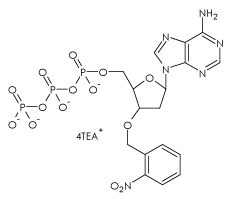
\includegraphics[width=2in]{./resources/BdATP-Structure.png}
\caption{\BdATP{}}
\label{bdatp}
\end{figure}
\section{Overview} % CHANGE THIS 
This lab will attempt to append \BdATP{} to a \textbf{short (25bp) primer}. The effectiveness of this attempt will be determined by attempting to form a homopolymer on the modified primer. If a homopolymer is formed, the blocking groups did not effectively prevent their formation. This could be due to many reasons (the most likely of which being that the blocking groups either (1) were appended without the 2' nitrobenzyl due to sample degradation or (2) were not appended). If the homopolymer was not formed (but a homopolymer was formed on the controls) it follows that the blocking groups prevented the formation of the homopolymer, likely due to them preforming their intended function. Moreover, all samples will be run on a PAGE gel in order to achieve single nucleotide resolution. This will allow us to confirm that the \BdATP{} is the only base appended to the "blocked" sample. A ddATP control will help as well.

% Safety First! ALSO, % CHANGE THIS
\section{Safety Information}
\begin{safety}
\begin{enumerate}
\SYBRGOLD{} % For select reagents, I've created custom commands so we don't have to copy and paste every time :)
\tdtSafety{}
\item{Working in a communal lab space is dangerous. Do not assume your fellow workers cleaned up sufficiently}
\end{enumerate}
\end{safety}

\section{Materials}
\begin{itemize}
\item{Primer (25bp)}
\item{100mM \BdATP{} Stock}
\item{10mM dNTP Stock}
\item{100mM dATP Stock}
\item{10mM ddATP Stock}
\item{5X \tdt{} Buffer}
\item{\tdt{} Stock (20U/\uL{})}
\item{Nuclease Free Water}
\item{TBE Buffer}
\item{20\% Urea Denaturing Gels}
\item{SYBR Gold}
\end{itemize}
% Now for the _good_ stuff  

\section{Procedure}% CHANGE THIS
\subsection{Sample Preparation}
\begin{figure}[ht]
\begin{center}
\begin{tabular}{ c | l }
	\hline
	A & The primer incubated with \textbf{dATP} and then commercial \textbf{dNTPs} \\
	B1 & The primer incubated with \textit{just} \textbf{NBdATP} \\
	B2 & The primer incubated with \textbf{NBdATP} and then \textbf{dNTPs}\\
	C & The primer incubated with just \textbf{dNTPs} in the second incubation \\
	D & The primer incubated with \textbf{ddATP} nucleotides and then \textbf{dNTPs} \\
	X & The primer incubated with \textbf{dNTPs} but \textbf{no \tdt{}} in the second incubation \\
	\hline
\end{tabular}
\end{center}
	\label{sampleTable}
	\caption{Samples and their experimental conditions}
\end{figure}
\begin{enumerate}
\item{Remove \BdATP{}, \tdt{}, primer, \tdt{}  buffer, ddATP stock and dATP stock from -20\C{} freezer}
\item{Let \BdATP{} thaw on ice in dark}
\item{Other reagents can thaw on ice in the light}
\subsection{Attempted blocking}
\item{Label three PCR Tubes A, B and D, respectively}
\item{Pipette 11\uL{} of nuclease free water into tube A}
\item{Pipette 13.7\uL{} of nuclease free water into tube B}
\item{Pipette 11\uL{} of nuclease free water into tube D}
\item{Pipette 4.0\uL{} 5X \tdt{} reaction buffer into all three PCR Tubes}
\item{Dilute Nucleotides:
\begin{enumerate}
\item{Label a PCR Tube "dATP Dilute"}
\item{Pipette 9\uL{} of nuclease free water into PCR Tube}
\item{Pipette 1\uL{} of dATP stock into PCR Tube}
\item{Vortex directly before use}
\end{enumerate}
}
\item{Pipette 0.5\uL{} of primer into all three PCR Tubes}
\item{Pipette 3\uL{} of dATP dilute into PCR Tube A}
\item{Pipette .3\uL{} of \BdATP{} stock into PCR Tube B}
\item{Pipette 3\uL{} of ddATP \textbf{10mM stock} into PCR Tube D}
\item{Gently pipette 1.5\uL{} \tdt (20U/\uL{}) into both PCR tubes.}
\item{Incubate sample at 37\C{} for 30 minutes}\\
\textbf{Note}: \textbf{Do NOT} deactivate \tdt{} 
\stopPoint{} 
\subsection{Extending}
Based off of our standard \tdt{} extending procedure \cite{genTdT}.
\item{Label two PCR Tubes C and X, respectively}
\item{Pipette 14\uL{} nuclease free water into PCR Tube C (see above, \textbf{ATTEMPTED BLOCKING})}
\item{Pipette 15.5\uL{} of nuclease free water into PCR Tube X (see above, \textbf{CONTROLS})}
\item{Pipette 0.5\uL{} of primer into both PCR Tubes}
\item{Set PCR Tube X aside.}
\item{Pipette 4.0\uL{} 5X \tdt{} reaction buffer into PCR Tube C}
\item{Pipette 3\uL{} of dNTP stock into PCR Tubes C and X}
\item{Pipette .4\uL{} of dNTP stock into PCR Tubes \textbf{A, B}}
\item{Wait until the previous samples have finished incubating}
\item{Label a PCR Tube "B1"}
\item{Pipette 10\uL{} from B into B1}
\item{Pipette 1.5\uL{} EDTA into \textbf{B1} to stop the reaction \cite{Invitrogen2002}}
\item{Gently pipette 1.5\uL{} \tdt{} (15 U/\uL{}) into \textbf{PCR Tube C}}
\item{Incubate \textbf{all} samples \textbf{except B1} at 37\C{} for 30 minutes}
\item{Pipette 1.5\uL{} nuclease free water into B1}
\item{Place B1 into -20\C{} freezer for later use}
\item{Stop any \tdt action by adding 2\uL{} 0.5M EDTA to the all PCR tubes \textbf{except B2} after incubation.\cite{Invitrogen2002}}
\item{Pipette 1\uL{} 0.5M EDTA into B2}
\RstopPoint{} 
\subsection{Analysis}
\subsection{XCell Surelock Setup and Pre-Run}
\item{Remove 20\% polyacrylamide gel from pouch and rinse with deionized water.}
\item{Peel off tape on bottom of 20\% polyacrylamide gel and remove the comb.}
\item{Gently wash every cassette well with 1X TBE buffer. Invert to remove buffer and shake. Repeat twice.}
\item{Lower the Buffer Core (the piece that holds the gels) into the Lower Buffer Chamber so that the negative electrode fits into the opening in the gold plate.}
\item{Insert the Gel Tension Wedge into the XCell Surelock behind the buffer core. Make sure it is in its 'unlocked' position, which allows the wedge to slip into the unit.}
\item{Insert gel cassettes into the lower buffer chamber. The shorter "well" side of the cassette faces into the buffer core. The slot on the back must face outward. If only one gel is being run, insert a buffer dam in the place of a gel cassette.}
\item{Pull forward on the Gel Tension Lever toward the buffer core until the gel cassettes are snug against the buffer core. This puts it in the 'locked' position.}
\item{Fill the Upper Buffer Chamber (between the gels) with running buffer. Ensure it is not leaking.}
\item{Fill the Lower Buffer Chamber completely with running buffer by pouring TBE next to the Gel Tension Wedge.}
\item{Pipette 12\uL{} of running buffer into each gel well.}
\item{Place the gel cover on the apparatus in the correct orientation. Connect the electrodes to the power source, and pre-run the gel for 30 minutes at 150V.}
\item{When there is only 5 minutes left on the incubation, retreive sample B1 from the freezer and let thaw on ice}
\subsubsection{Run Gel}
\begin{figure}[ht] %This is a figure, in this case, a well plate
\begin{center} 
\begin{tabular}{|l|l|}
\hline
Well number				& Sample \\ \hline
\rownumber                                 & 10/60 DNA Ladder   \\ \hline
\rownumber				   & Custom Ladder (40ng) \\ \hline
\rownumber                                 & B1 (40ng)\\ \hline
\rownumber                                 & B2 (40ng)\\ \hline
\rownumber                                 & X (40ng) \\ \hline
\rownumber                                 & X + B1  (40ng each)\\ \hline
\rownumber                                 & X + B2  (40ng each)\\ \hline
\rownumber				   & D (40ng)	\\ \hline
\rownumber                                 & X + D (40ng each)	\\ \hline
\rownumber                                 & A (40ng)	\\ \hline
\rownumber                                 & C (40ng)  \\ \hline
\rownumber                                 & 26-Mer (40ng) \\ \hline
\rownumber                                 & 25-Mer (40ng) \\ \hline % to see if we have bad separation between lanes like the last procedure
\rownumber                                 & Custom Ladder (40ng)     \\ \hline
\rownumber                                 & 10/60 DNA Ladder  \\ \hline

\end{tabular}
\label{tab:Gel Layout} %Label your stuff, this is for referencing in the future
\caption{Wells} %Caption!
\end{center}
\end{figure}
\textbf{Note}: Be relatively swift about mixing and loading, as the samples will gradually begin to evaporate if left on the parafilm for too long.
\item{Obtain a sizable piece of parafilm. Pipette 3 \uL{} of Gel Loading Buffer in a row of 15 droplets.}
\item{For the 10/60 Ladder samples, pipette 1uL of 10/60 Ladder and 4 uL of running buffer and mix.}
\item{For the remaining droplets, add 3 \uL{} of the appropriate sample. See the corresponding table (Figure \ref{tab:Gel Layout}) above for sample location and order.}
\item{As you go, pipette up and down to mix thoroughly.}
\item{Load the gels (with 5 \uL{} sample in each well) when they are finished pre-running. Ensure pipette tip is fully in the well, and depress slowly and carefully. Work quickly to minimize diffusion.}
\item{Run the gel(s) at 150V until the dark blue dye is at the bottom.}

\subsubsection{Stain \& View Gel}
\item{While the gel runs, prepare 1X SYBR Gold Staining Solution with TBE as dilute}
	\begin{enumerate}
		\item{Add 6\uL{} SYBR Gold to 60\uL{} of TBE running buffer}
	\end{enumerate}
\item{Once gel has finished running, \textbf{\textit{lightly}} agitate gel while submerged in solution for 60 minutes.}
\item{Review gel with gel viewer. Until unnecessary, place gel back in stain for 20 minute increments and re-image.}
\item{Post pictures to Slack.}\\
\end{enumerate} 

% Stop Procedure
\section*{Stop Procedure}
\begin{enumerate}
\item{Pipette samples into PCR tubes if not already contained in an appropriate manner}
\item{Label containers if not already labeled}
\item{Freeze samples at -20\C{}}
\end{enumerate}

\bibliographystyle{ieeetr}
\bibliography{main}
\end{document}
